\section{数値解析例}
本節では,Na型モンモリロナイトに対する水和エネルギーを用いて行った
CG-MDシミュレーションの結果を示す.ここでは,非平衡状態にある
モンモリロナイト含水系(以下,単に粘土含水系と呼ぶ)の初期モデルから,
温度,相対湿度,圧力を一定に保った緩和計算を行う.
これを6つの異なる相対湿度において行い,層間距離や粘土分子配置の変化を調べる.
以下では,初期モデルの準備を含む計算手順を述べた後,シミュレーション結果を
粘土分子配置のスナップショットと層間距離の頻度分布として示す。
これらの結果をもとに,相対湿度に応じて組織構造にどのような差が見られるかを述べる.
\subsection{初期モデルの作成}
初期モデルを図\ref{fig:fig3}-(a)に示す.
これは2021年度の共同研究報告書で述べた方法で作成した
粘土含水系モデルの一つである.粘土含水系を構成する
分子数は80で,合計の粗視化粒子数は3,194となっている.
このモデルは以下の計算を経て得られたものである.\\
\hspace{\parindent}
はじめに,直線状の粘土分子を200$\times$200[nm$^2$]の矩形領域に,
互いに重ならないよう,位置と向きをランダムに配置する.
この矩形領域を周期構造の単位セルとして,乾燥密度が約1.6g/cm$^{3}$
となるまで断熱圧縮する.その際,粒子系の運動方程式を積分するための
時間ステップ幅は0.02[ps],時間ステップ数は5万ステップ,
時間範囲は1[ns]としており,時間ステッピングに関する
条件は以後の解析でも同じである.断熱圧縮過程では,
系の温度を制御しないため,圧縮によってに加えれられたエネルギーで
粘土含水系モデルは高い温度となり平衡状態にも無い.
そこで,圧縮後のモデルを300Kまで$250$psの間冷却し,
その後750ps温度を300Kに保ってで緩和計算を行う.
なお,ここでいう緩和とは,温度や体積などの外的条件を一定にして
系を平衡状態へ推移させることを意味する.
以上の計算では,各粗視化粒子が保持する水分量を表すパラメータである
粒子間相互作用ポテンシャルの特性距離$\sigma$は,
二層膨潤状態に相当する$\sigma=1.5$[nm]に固定している.
これは,系内での水分移動も系外との水分の授受も行わない
ことを意味する.最後に,無次元化された化学ポテンシャル$\bar \mu$
を$0.5$に保ち,温度,体積一定のもと,水分移動を許容した
緩和計算を1ns間行う.このとき$\bar \mu$の値は強い排水が起こるように
設定されているため,緩和計算後は,比較的大きな層外空隙をもつ
組織構造が得られる.\\
\hspace{\parindent}
図\ref{fig:fig3}-(a)は,以上の方法で得られた粘土含水系モデルである.
本年度の研究では,これを初期構造とし,Na型モンモリロナイトの
水和エネルギーモデルを用いて,相対湿度一定での緩和計算を行う.
なお,初期構造を得るまでの計算では,昨年度の研究で検討した
水和エネルギーモデルの一つである振動モデルを用いている.
このモデルは仮想的な粘土の水和挙動を表現したものであるため,
図\ref{fig:fig3}-(a)の状態は,今回新たに作成した水和エネルギー
モデルの下では平衡状態にない.そのため,相対湿度の設定値によらず,
水分や分子配置には必ず何らかの変化が生じる.
%%%%
\subsection{相対湿度50$\%$に対する結果}
図\ref{fig:fig3}の(b)と(c)は,相対湿度50$\%$,温度300K, 圧力10MPaで
1ns間,緩和計算を行ったときの粘土分子配置の変化を示したものである.
(b)は経過時間が250psの時点での配置を,(c)は1nsで緩和計算を終了した
時点の結果を示している.
初期状態(a)では水分量が少ないため,緩和計算初期の段階で速やかに
吸水が起こり,(b)では積層間隔が拡がった結果,A-Dのラベルで示した
層外間隙の量が(a)よりも減少している.
一方,(b)から(c)の間には,粘土分子の配置にあまり大きな変化は
なく,(b)の時点から安定した構造が形成されていることがうかがわれる.
ただし,間隙Aの収縮は(b)から一層進行し,(c)の図ではほぼ消失している.
これに対して,粘土分子を巻き込むことで形成された層外間隙の
CとDは,吸水に伴う層間距離の拡張で生じる収縮は比較的小さく,
水分量の変化に対し組織構造を維持する役割を果たしていると推察される.
また,この計算では領域全体の体積は拘束されていないため,
初期状態(a)から(b)を経て(c)に移行する過程で,若干全体としての
体積収縮が認められる.このように,吸水による層間距離の拡張がある場合も,
層外間隙の収縮が勝り,全体としては収縮がおきることもあり得る点は,
マクロスコピックな膨潤挙動について考える際にも留意すべき点と考えられる.
%--------------------
\begin{figure}[t]
	\begin{center}
	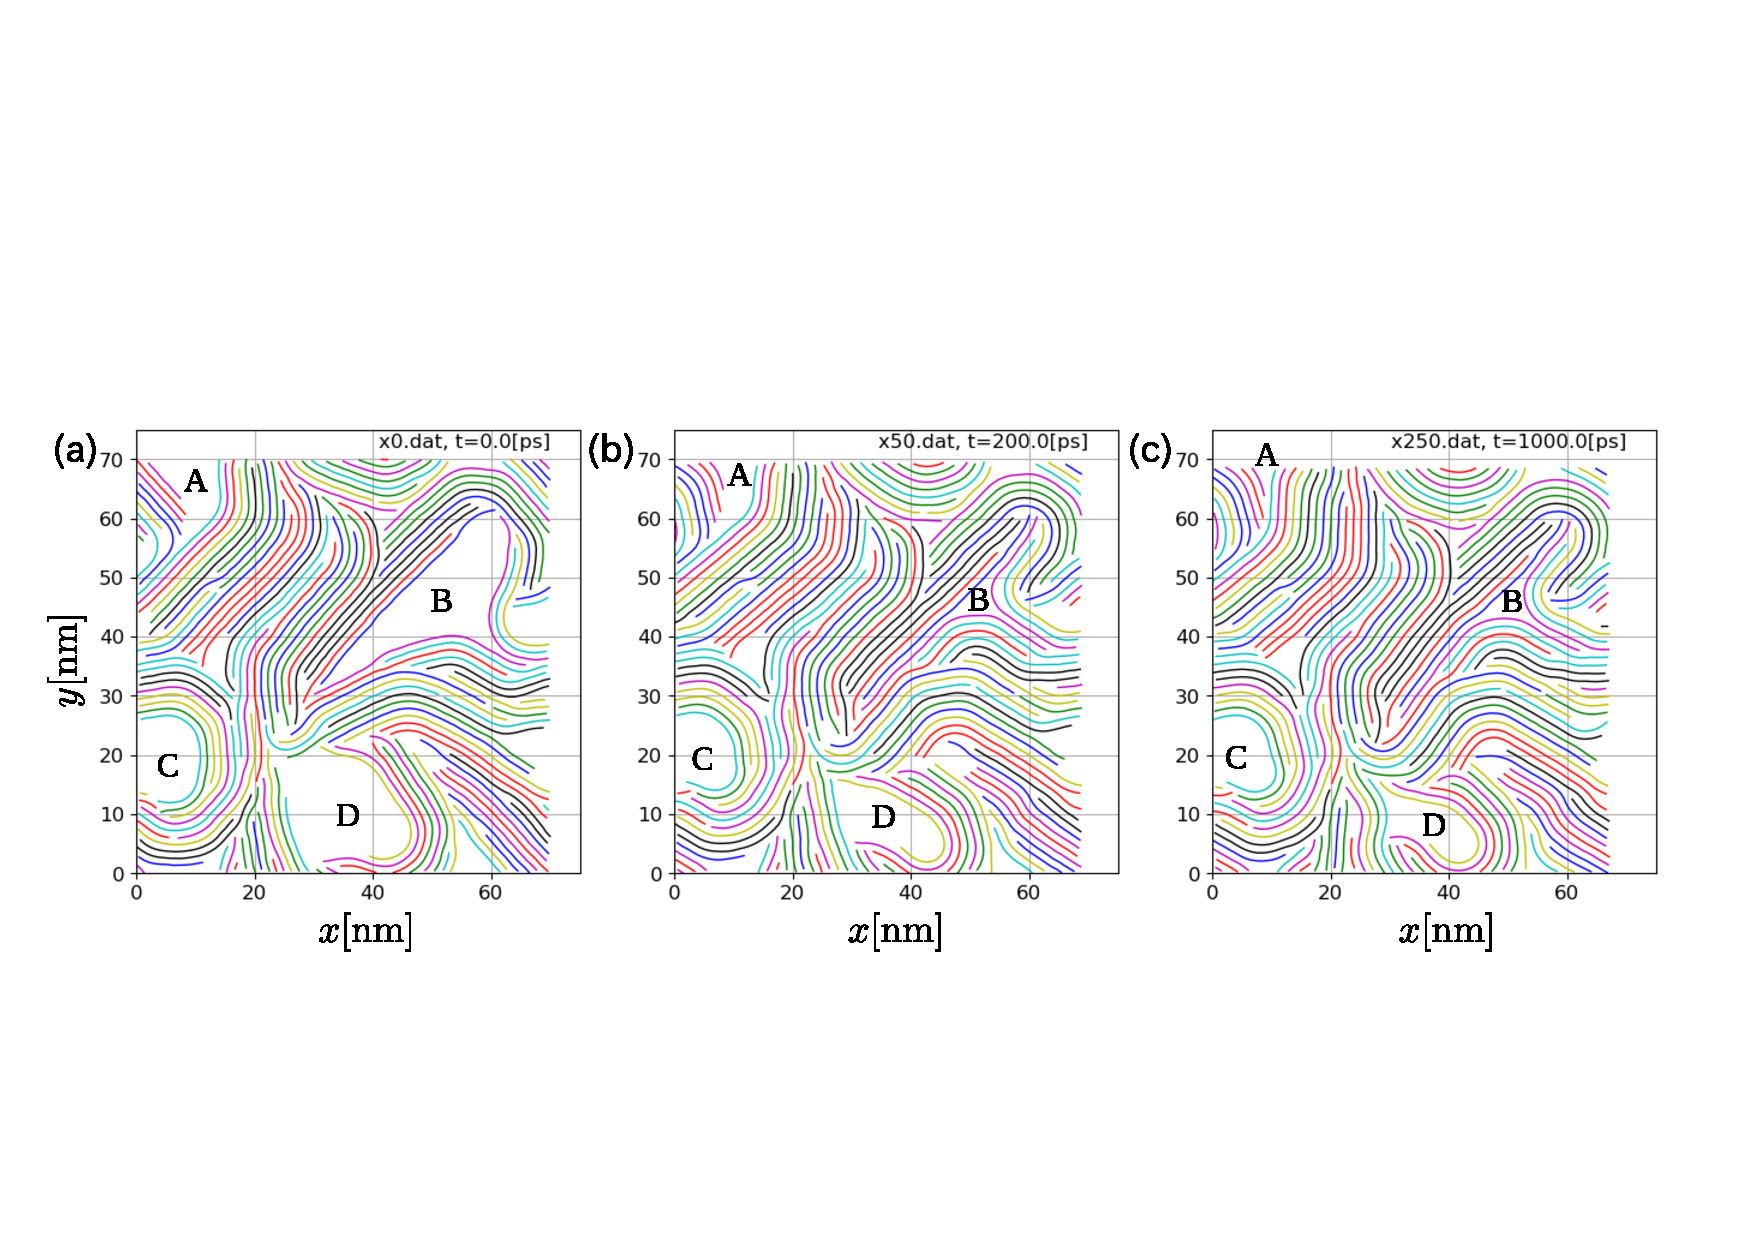
\includegraphics[width=1.0\linewidth]{Figs/fig3.pdf} 
	\end{center}
	\caption{
		相対湿度50$\%$での緩和にともなう粘土分子配置の変化.  
		(a)は初期状態,(b)緩和開始から200psの状態,(c)は1ns経過後の最終状態.
		A-Dのラベルは粘土層外の主要な間隙を示す.
	} 
	\label{fig:fig3}
\end{figure}
%--------------------
\begin{figure}[h]
	\begin{center}
	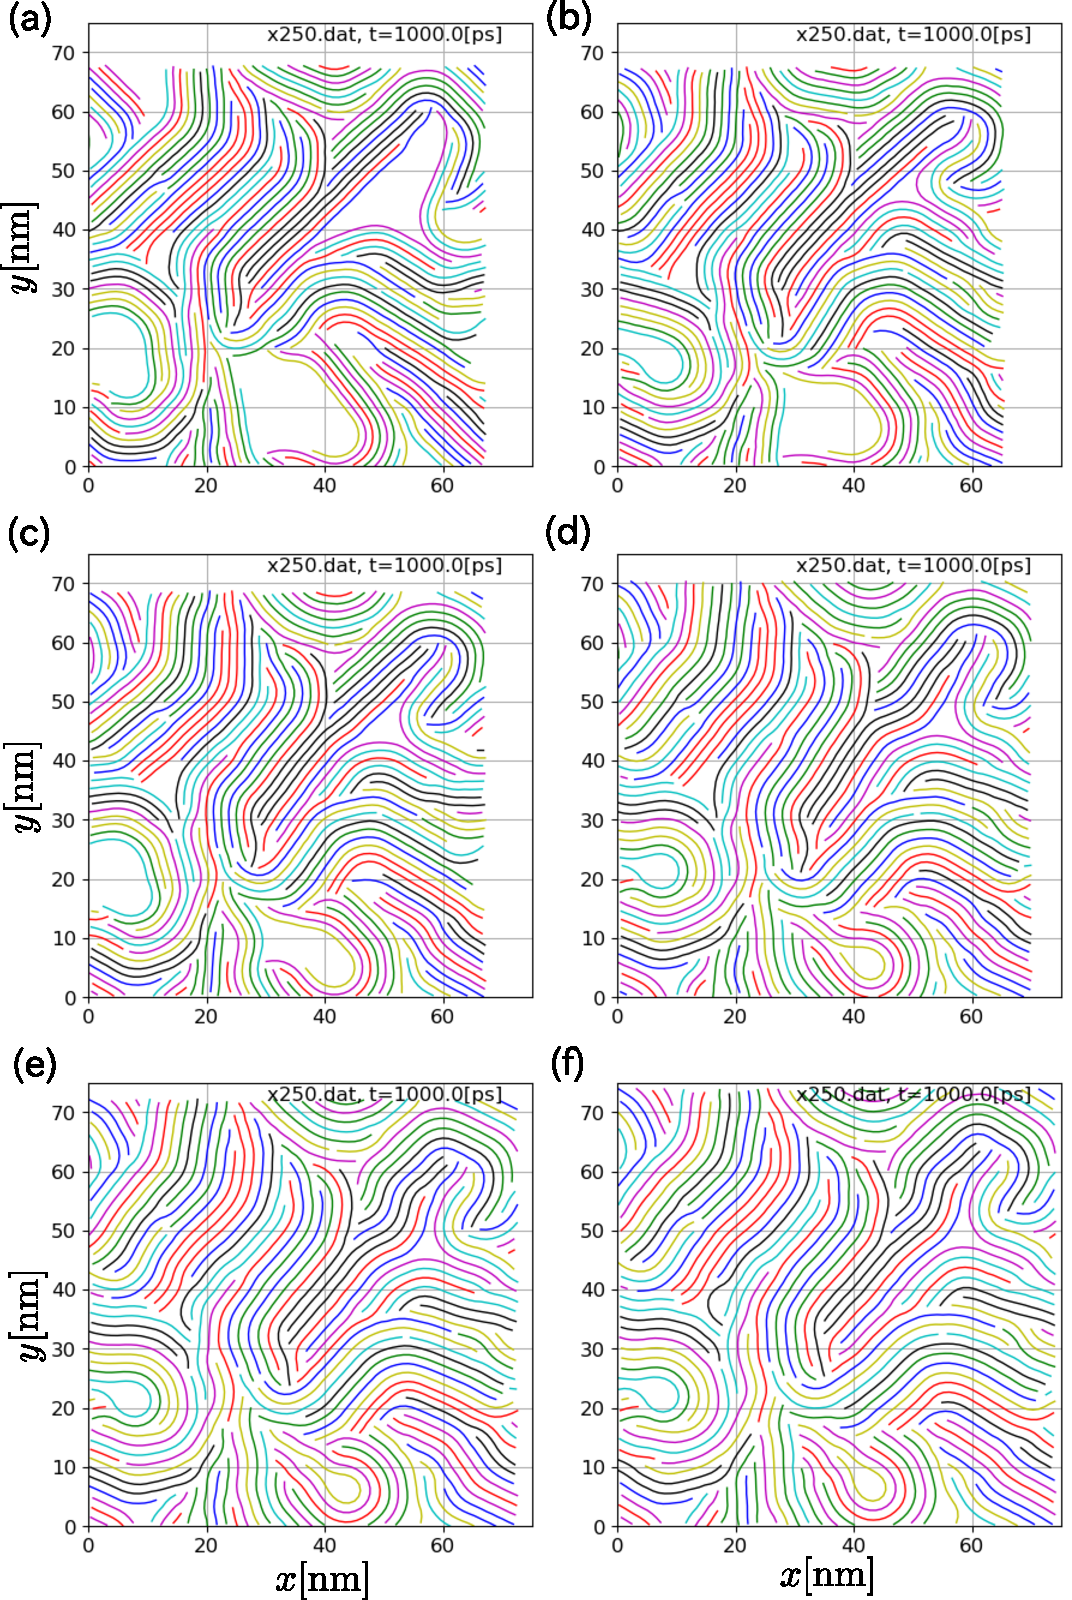
\includegraphics[width=0.7\linewidth]{Figs/fig4.pdf} 
	\end{center}
	\caption{
		6つの異なる相対湿度において得られた粘土含水系の組織構造.
		相対湿度は(a)から(f)の順に10,20,50,65,75および90$\%$. 
		相対湿度50$\%$の結果は,図\ref{fig:fig3}-(c)と同じものを再掲.
	} 
	\label{fig:fig4}
\end{figure}
\subsection{相対湿度による組織構造の違い}
ここまでに示した相対湿度50$\%$の場合に加えて,
10,20,65,75および90$\%$で緩和計算を行った結果を
図\ref{fig:fig4}に示す.なお,これらの計算において,
相対湿度以外の計算条件は前項50$\%$の場合と同じである.\\
\hspace{\parindent}
図\ref{fig:fig4}のうち,相対湿度が最も低い(a)10$\%$の
ケースでは,初期構造(図\ref{fig:fig3}-(a))からあまり
変化がなく,層外間隙の形や大きさはも当初と同程度の
ままになっている.これは,初期構造が相対湿度$10\%$程度の
低い場合に生じるものであったことを意味する.
ただし,系全体の体積はやや初期状態から収縮しており,
若干の排水が生じていることが予想される.2番目に低い
相対湿度である(b)20$\%$では,全体体積は(a)と同程度の
収縮を起こしている.また,初期構造から大きく収縮する
層外間隙もあり,相対湿度50$\%$(図\ref{fig:fig3}-(c)と図\ref{fig:fig4}-(c))
によく似た分子配置となっている.
ただし(c)$50\%$のケースと比べると,初期状態からの
系全体の収縮量は(b)の方が大きく,(b)から(c)の
相対湿度範囲では次第に吸水の効果が大きくなりつつある
と解釈できる.これに対して(d)65$\%$の場合,
全体としての体積変化はほぼ無視できる程度だが,
粘土層間の距離は(b)や(c)の場合より大きく,
吸水による膨張の効果が系全体に及びはじめている.
この段階では粘土分子の巻き込みで残留した層外空隙も
かなりの程度圧縮が進んでいる.さらに相対湿度の高い
(e)75$\%$と(f)90$\%$では,系全体としても膨張し始め,
このことは,層外間隙の体積収縮が(d)のケース
以上には大きく進行しないことと呼応している.\\
\hspace{\parindent}
相対湿度と膨潤状態の関係をより詳しく調べるために,
層間距離の相対湿度による変化をみる.
図\ref{fig:fig5}はその目的のために,
層間距離の頻度分布を相対湿度毎に示したものである.
これらのグラフは,横軸が層間距離を縦軸が頻度を示している.
CG-MD法では,粒子間相互作用を規定するレナード-ジョーンズ
ポテンシャルの特性距離$\sigma$で水分量を表現している.
$\sigma$は,概ね,粘土分子が積層したときの層間距離となるため,
$\sigma$を層間距離とみなし, その頻度分布を描いたのが
図\ref{fig:fig5}である. 横軸の範囲は,10から16$\AA$としており,
縦軸はグラフ毎に適切なサイズに描画されるように設定している.
なお,図\ref{fig:fig1}-(a)にもあるように,系が気体状態の水
に接している状態では,これらの頻度分布に示した範囲外の
層間距離となることはない.また,無水状態である0膨潤で
層間距離は約10$\AA$,1および2層膨潤状態では,層間距離は
それぞれ12.5と15.5$\AA$である。ただし,図\ref{fig:fig1}-(a)から
も分かるように,天然のモンモリロナイトでは,0から2層までの
膨潤状態それぞれに対応す層間距離を厳密に定義することは難しく,
上に挙げた層間距離は代表値と考えることがより実情にあう.\\
\hspace{\parindent}
図\ref{fig:fig5}に示されるように,全体としては
相対湿度の増加にともない,頻度分布の山は右方向に移り
層間距離が大きくなる傾向があることは明らかである.
ただし,分布幅と形状は相対湿度によって異なり,
相対湿度が低いときと,複数のピークが現れる場合に
分布幅が大きくなる傾向がある.
また,一つ一つ相対湿度における分布に関しては,以下のことが読み取れる.\\
\hspace{\parindent}
相対湿度が最も低い(a)の結果は,他の場合と比べて分布幅が明らかに広い.
このとき,層間距離は10$\sim$12$\AA$の間に分布し, 0層と1層膨潤の
中間的な状態になっている.2番目に相対湿度の低い(b)では,層間距離が
12$\AA$周辺に集中し,ほぼ1層膨潤状態に移行している.
図\ref{fig:fig1}-(a)を見ると,粉末X線回折試験では10$\sim$20$\%$の
相対湿度では層間距離は10$\AA$の0層膨潤となっているため,
CG-MD計算の方がより多くの水分が保持される結果となっている.
これは,(a)の状態から更に排水を進めるためには,すでに形成されている
粘土分子の積層構造を変形させる必要があるが,粉末状態の粘土と比べ
変形を生じさせるためにより多くのエネルギーが必要とされる
ことに起因したものと考えられる.
%狭い領域で積層した状態では変形が起こりにくく,水分を持つ方が,系全体の
%自由エネルギーを下げ,構造を安定させるためと考えられる.
%逆に言えば,指定された初期構造から0層膨潤状態に移行させるためには,
%より大きなエネルギーを加えて計全体を強く圧縮するか,組織構造
%を破壊する必要があることを示唆している.
これに対し,相対湿度50$\%$の結果(c)では,分布幅が狭く
層間距離がほぼ12.5$\AA$と決まる.この層間距離は粉末XRD試験の結果
と一致している.また,系全体としても体積膨張を起こすことなく水分が
取り込まれていることから,初期構造から到達および維持されやすい組織構造
になっていると考えられる.次に,(d)65$\%$と(e)75$\%$の結果を見ると,
3つあるいは2つピークをもつ多峰分布になっている.
粉末X線試験結果(図\ref{fig:fig1}-(a))をみると,これらの相対湿度は
1層から2膨潤への遷移領域にあたっている.
頻度分布における13$\AA$と15.5$\AA$付近のピークは,1層および2層膨潤
にそれぞれ対応している.14$\AA$付近にはピークが無いことから,
1層と2層膨潤が混在しているものの,中間的な膨潤状態は現れておらず,
Na型モンモリロナイトの離散的な膨潤挙動がシミュレーション結果に現れている.
ただし,(d)の結果では13$\AA$前後で大小2つのピークに分布が分離している.
大ピークは安定な1層膨潤状態にとどまっている層間水を,
小ピークは,既に2層へ移行が開始しつつあるものの,十分な水分が行き渡らず
1層膨潤に近い層間距離にとどまる箇所があることを意味している.
実際,大小のピークの谷間である13.1$\AA$は,図\ref{fig:fig1}-(a)に
ある膨潤曲線が大きく折れ曲がっており,この層間距離を境に,粉末試料でも
膨潤挙動が変化している.このことを踏まえれば,(d)よりやや相対湿度の
高い(e)で大ピークが消失していることは,全ての層間水が2層膨潤状態に
向かって移行を開始した状態にあると解釈できる.
最後に,最も相対湿度の高い(f)の場合は、2層膨潤への移行が終了し,
鋭いピークを持つ分布が現れている.そのピーク位置は15.5$\AA$で,
粉末X線回折試験結果で観察される層間距離とほとんど一致している.\\
\hspace{\parindent}
%なお,(d)に見られる第3の小ピークを伴う遷移挙動が実際の固体粘土で観察も
%現れるのか,
以上のように,今回のCG-MD計算に用いた水和エネルギーモデルでは,
1層から2層膨潤へは,Na型モンモリロナイトの粉末X線回折試験結果に見られる
離散的な膨潤挙動がよく現れている.
一方,湿度の低いケースでは,0層膨潤状態ははっきりと現れず,1層から0
層膨潤への移行が粘土分子の積層構造に妨げられる可能性があることが分かった.
このような挙動が実際の粘土でも現れるのか,またその影響がX線回折パターン
にも反映されるかは,メソスケール組織構造を実験によって調べる上で
興味深い問題の一つと思われる。
%--------------------
\begin{figure}[h]
	\begin{center}
	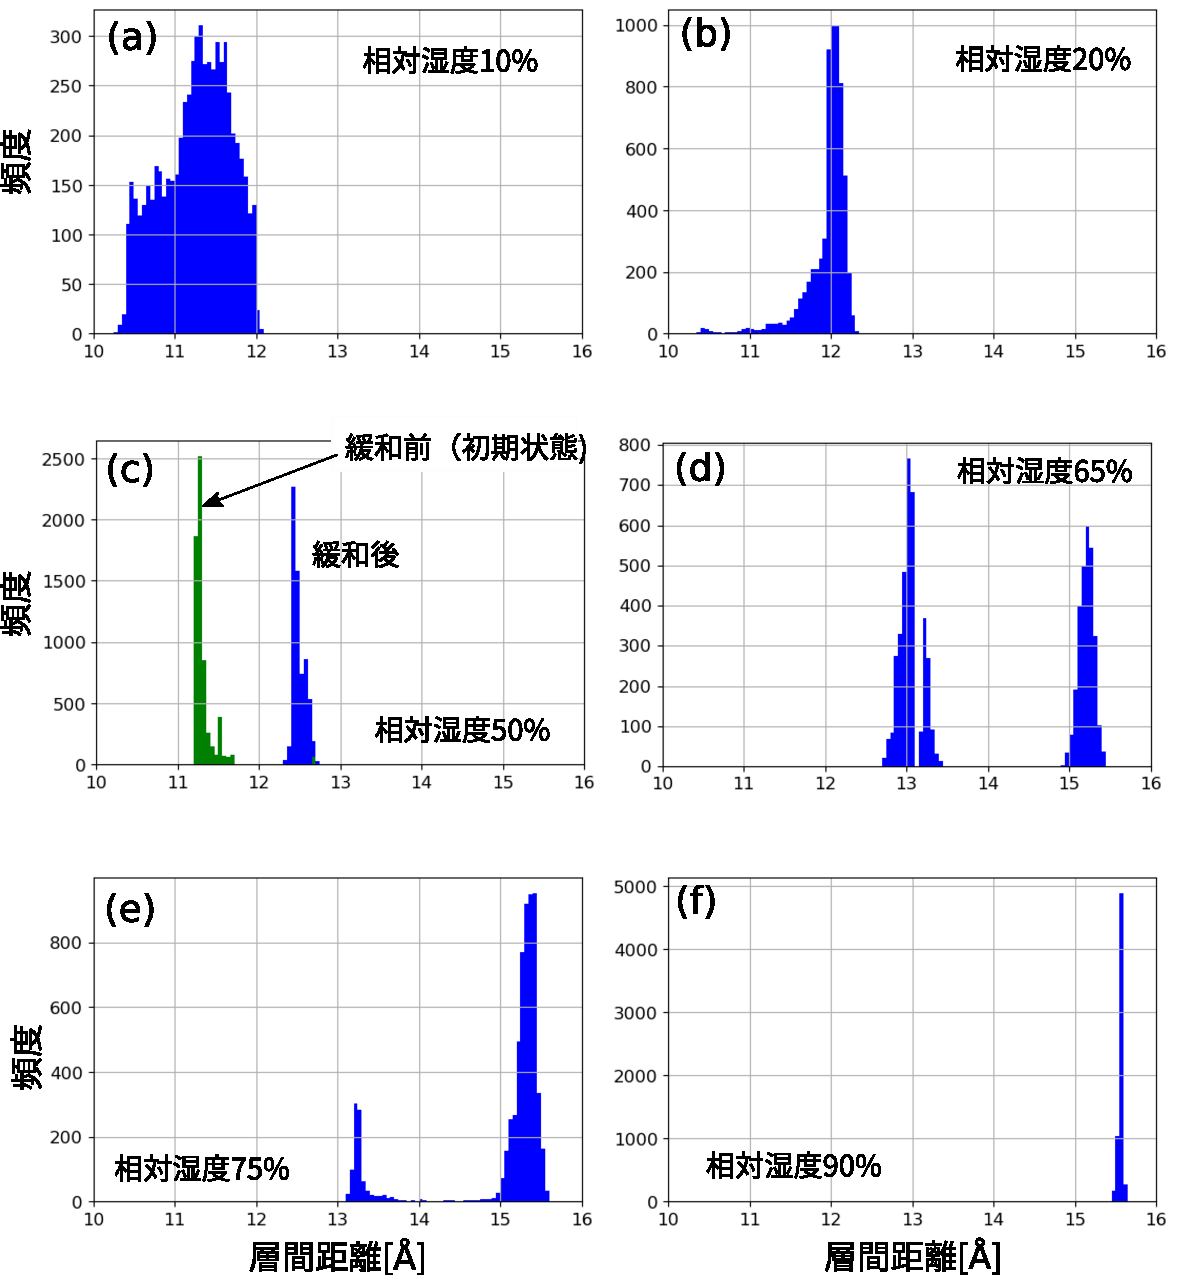
\includegraphics[width=1.0\linewidth]{Figs/fig5.pdf} 
	\end{center}
	\caption{
		6つの異なる相対湿度における層間距離の頻度分布.
		相対湿度は(a)から(f)の順に10,20,50,65,75および90$\%$. 
		(c)に示した緑の分布は,初期構造(緩和計算開始時)の
		層間距離の頻度分布を表す.
	} 
	\label{fig:fig5}
\end{figure}
%--------------------
